\documentclass{article}
\usepackage[a4paper, total={17cm,23.7cm}]{geometry}
\usepackage[utf8]{inputenc}
\usepackage{graphicx}
\usepackage[export]{adjustbox}
\usepackage{csvsimple}
\begin{document}
    \section*{Entfernungen}
    Bezugspunkt: Gabelung Portikus (direkt am RSV-Gelände). \\        
    \csvautotabular[separator=semicolon]{distances.csv}
    
    \section*{Anmerkungen}
    Die Entfernungen beziehen sich auf die in OpenStreetMap vorhandenen,
    repräsentativen Linien von Wasserläufen und ggf. hinzugefügte Routen auf
    Seen. Die Entfernungen sind sowohl auf der Karte als auch in der Tabelle auf 5~m gerundet.
    
    \newpage
    \section*{Karten}

    \begin{figure}[!h]
        \centering
        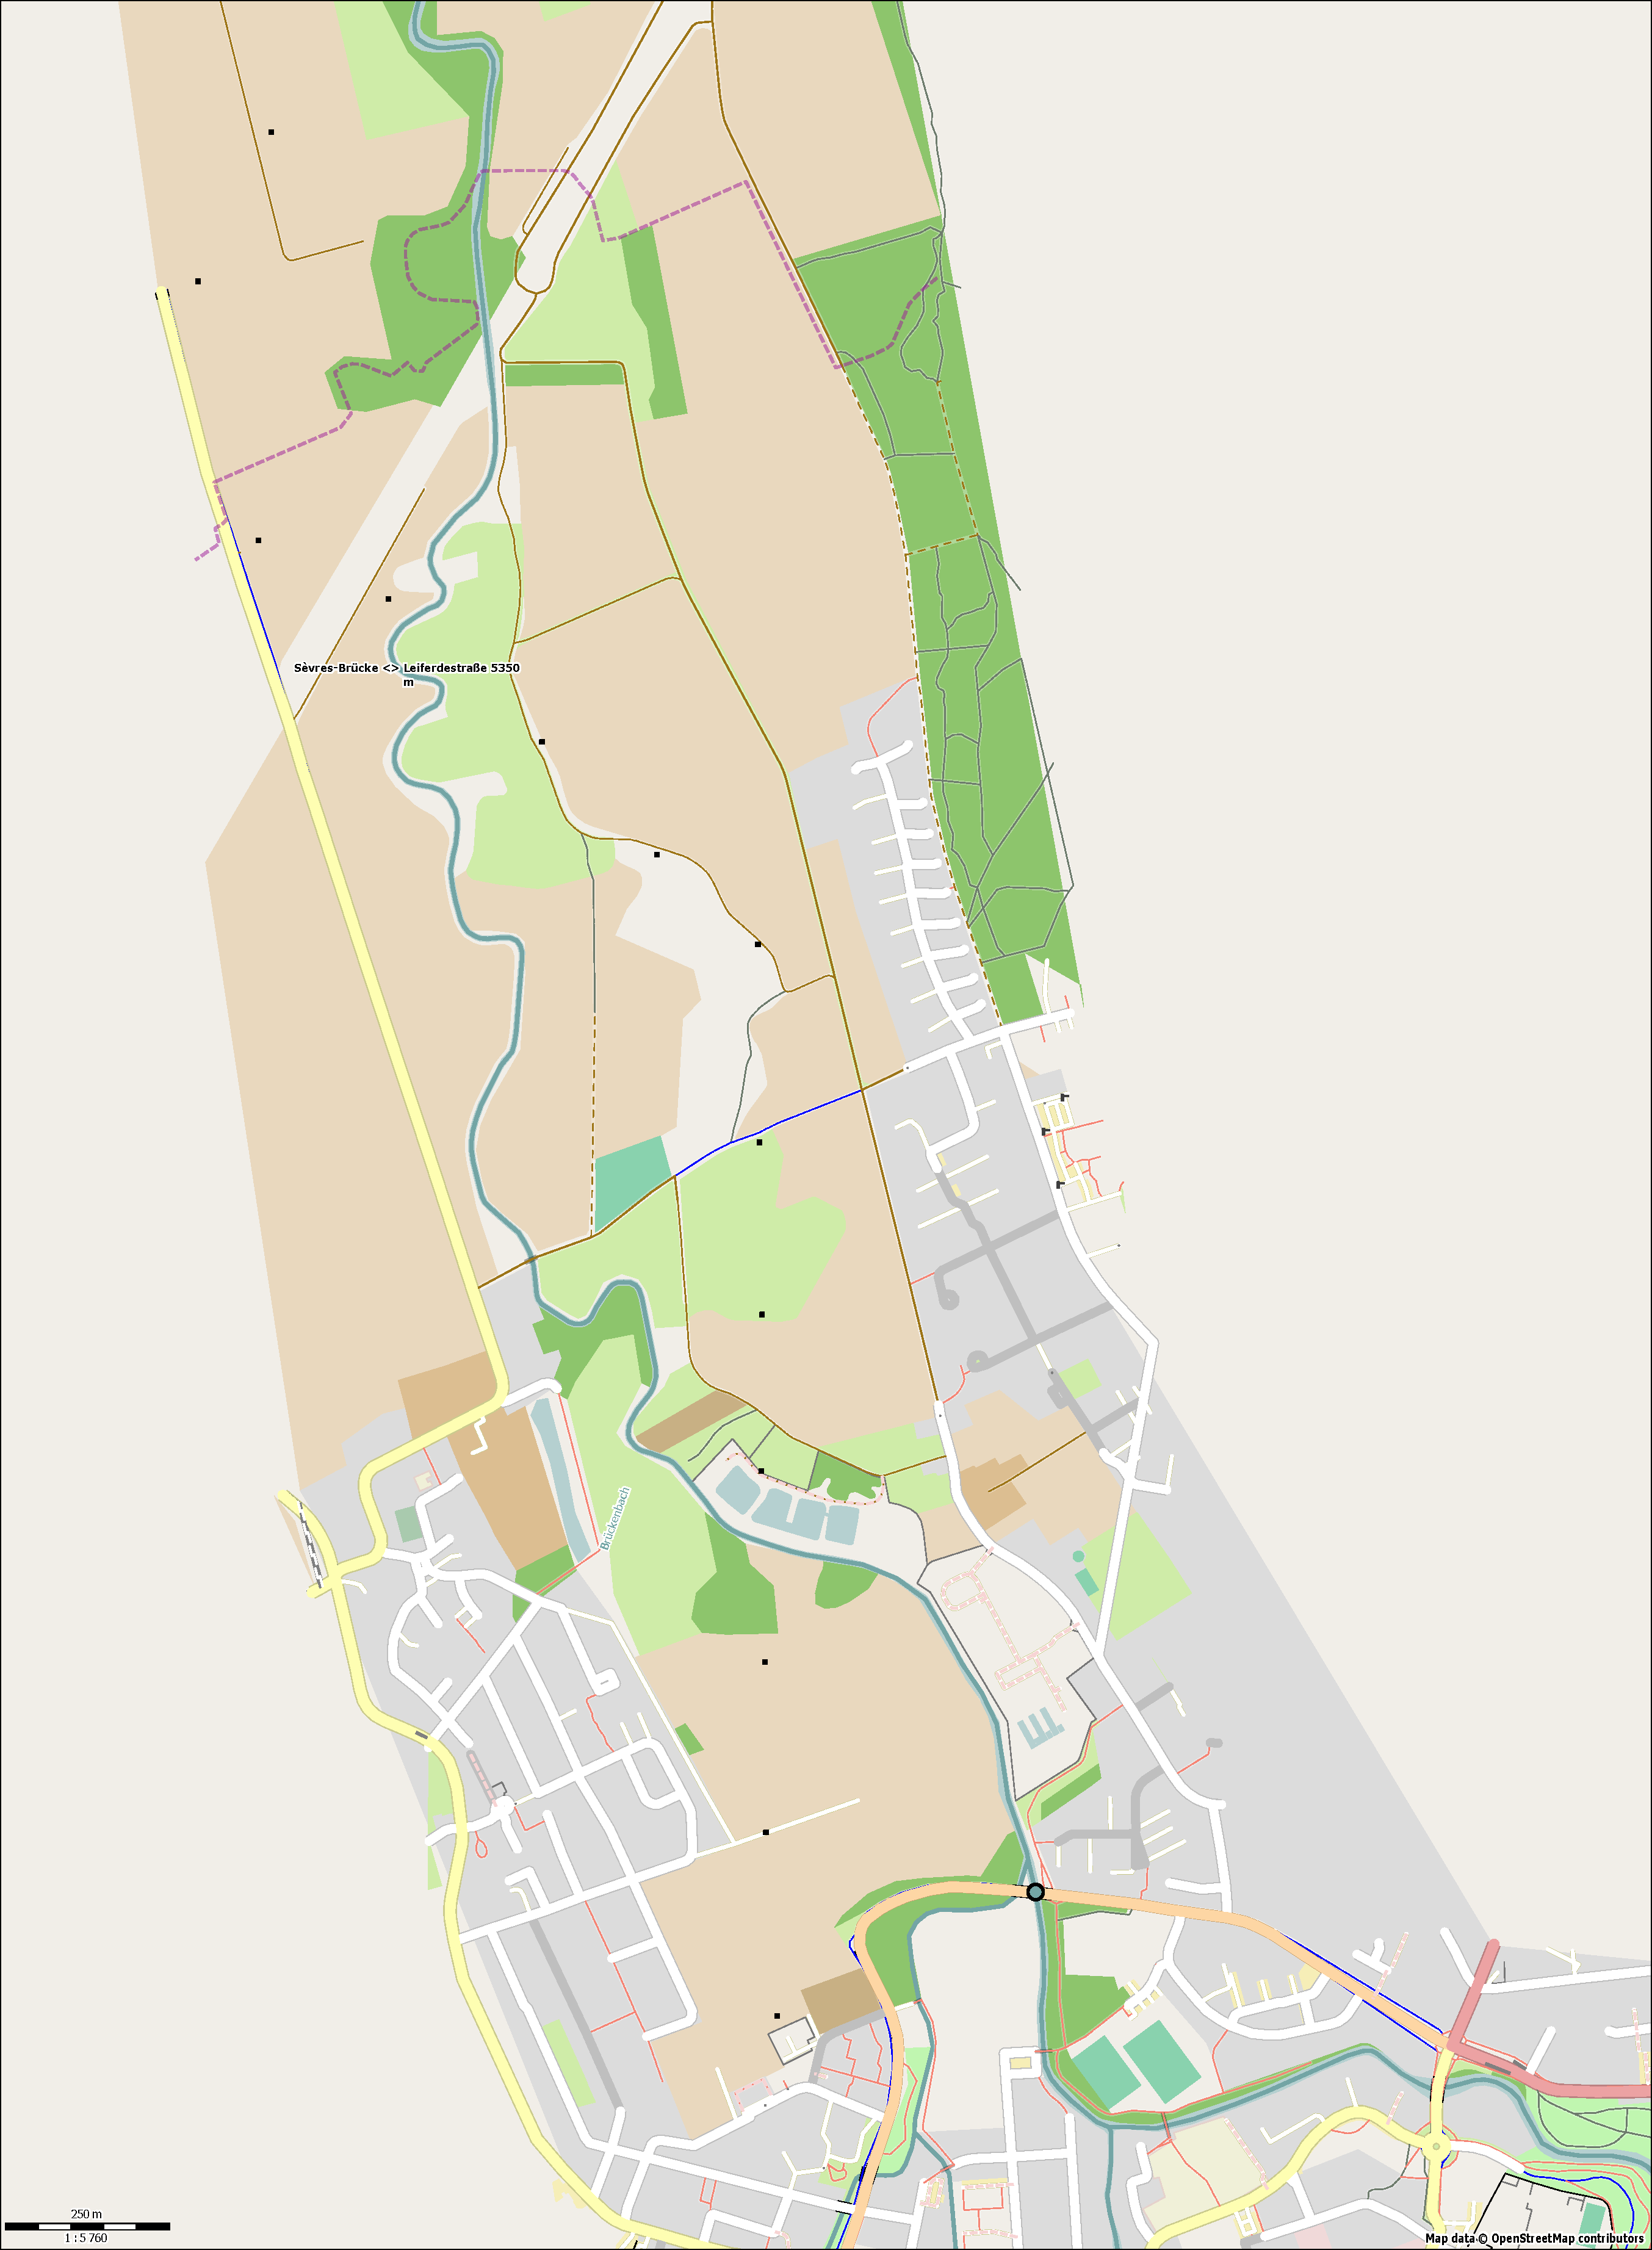
\includegraphics[max size={\textwidth}{\textheight}]{../Result/WF.pdf}
    \end{figure}
    \newpage
    
    \begin{figure}[!h]
        \centering
        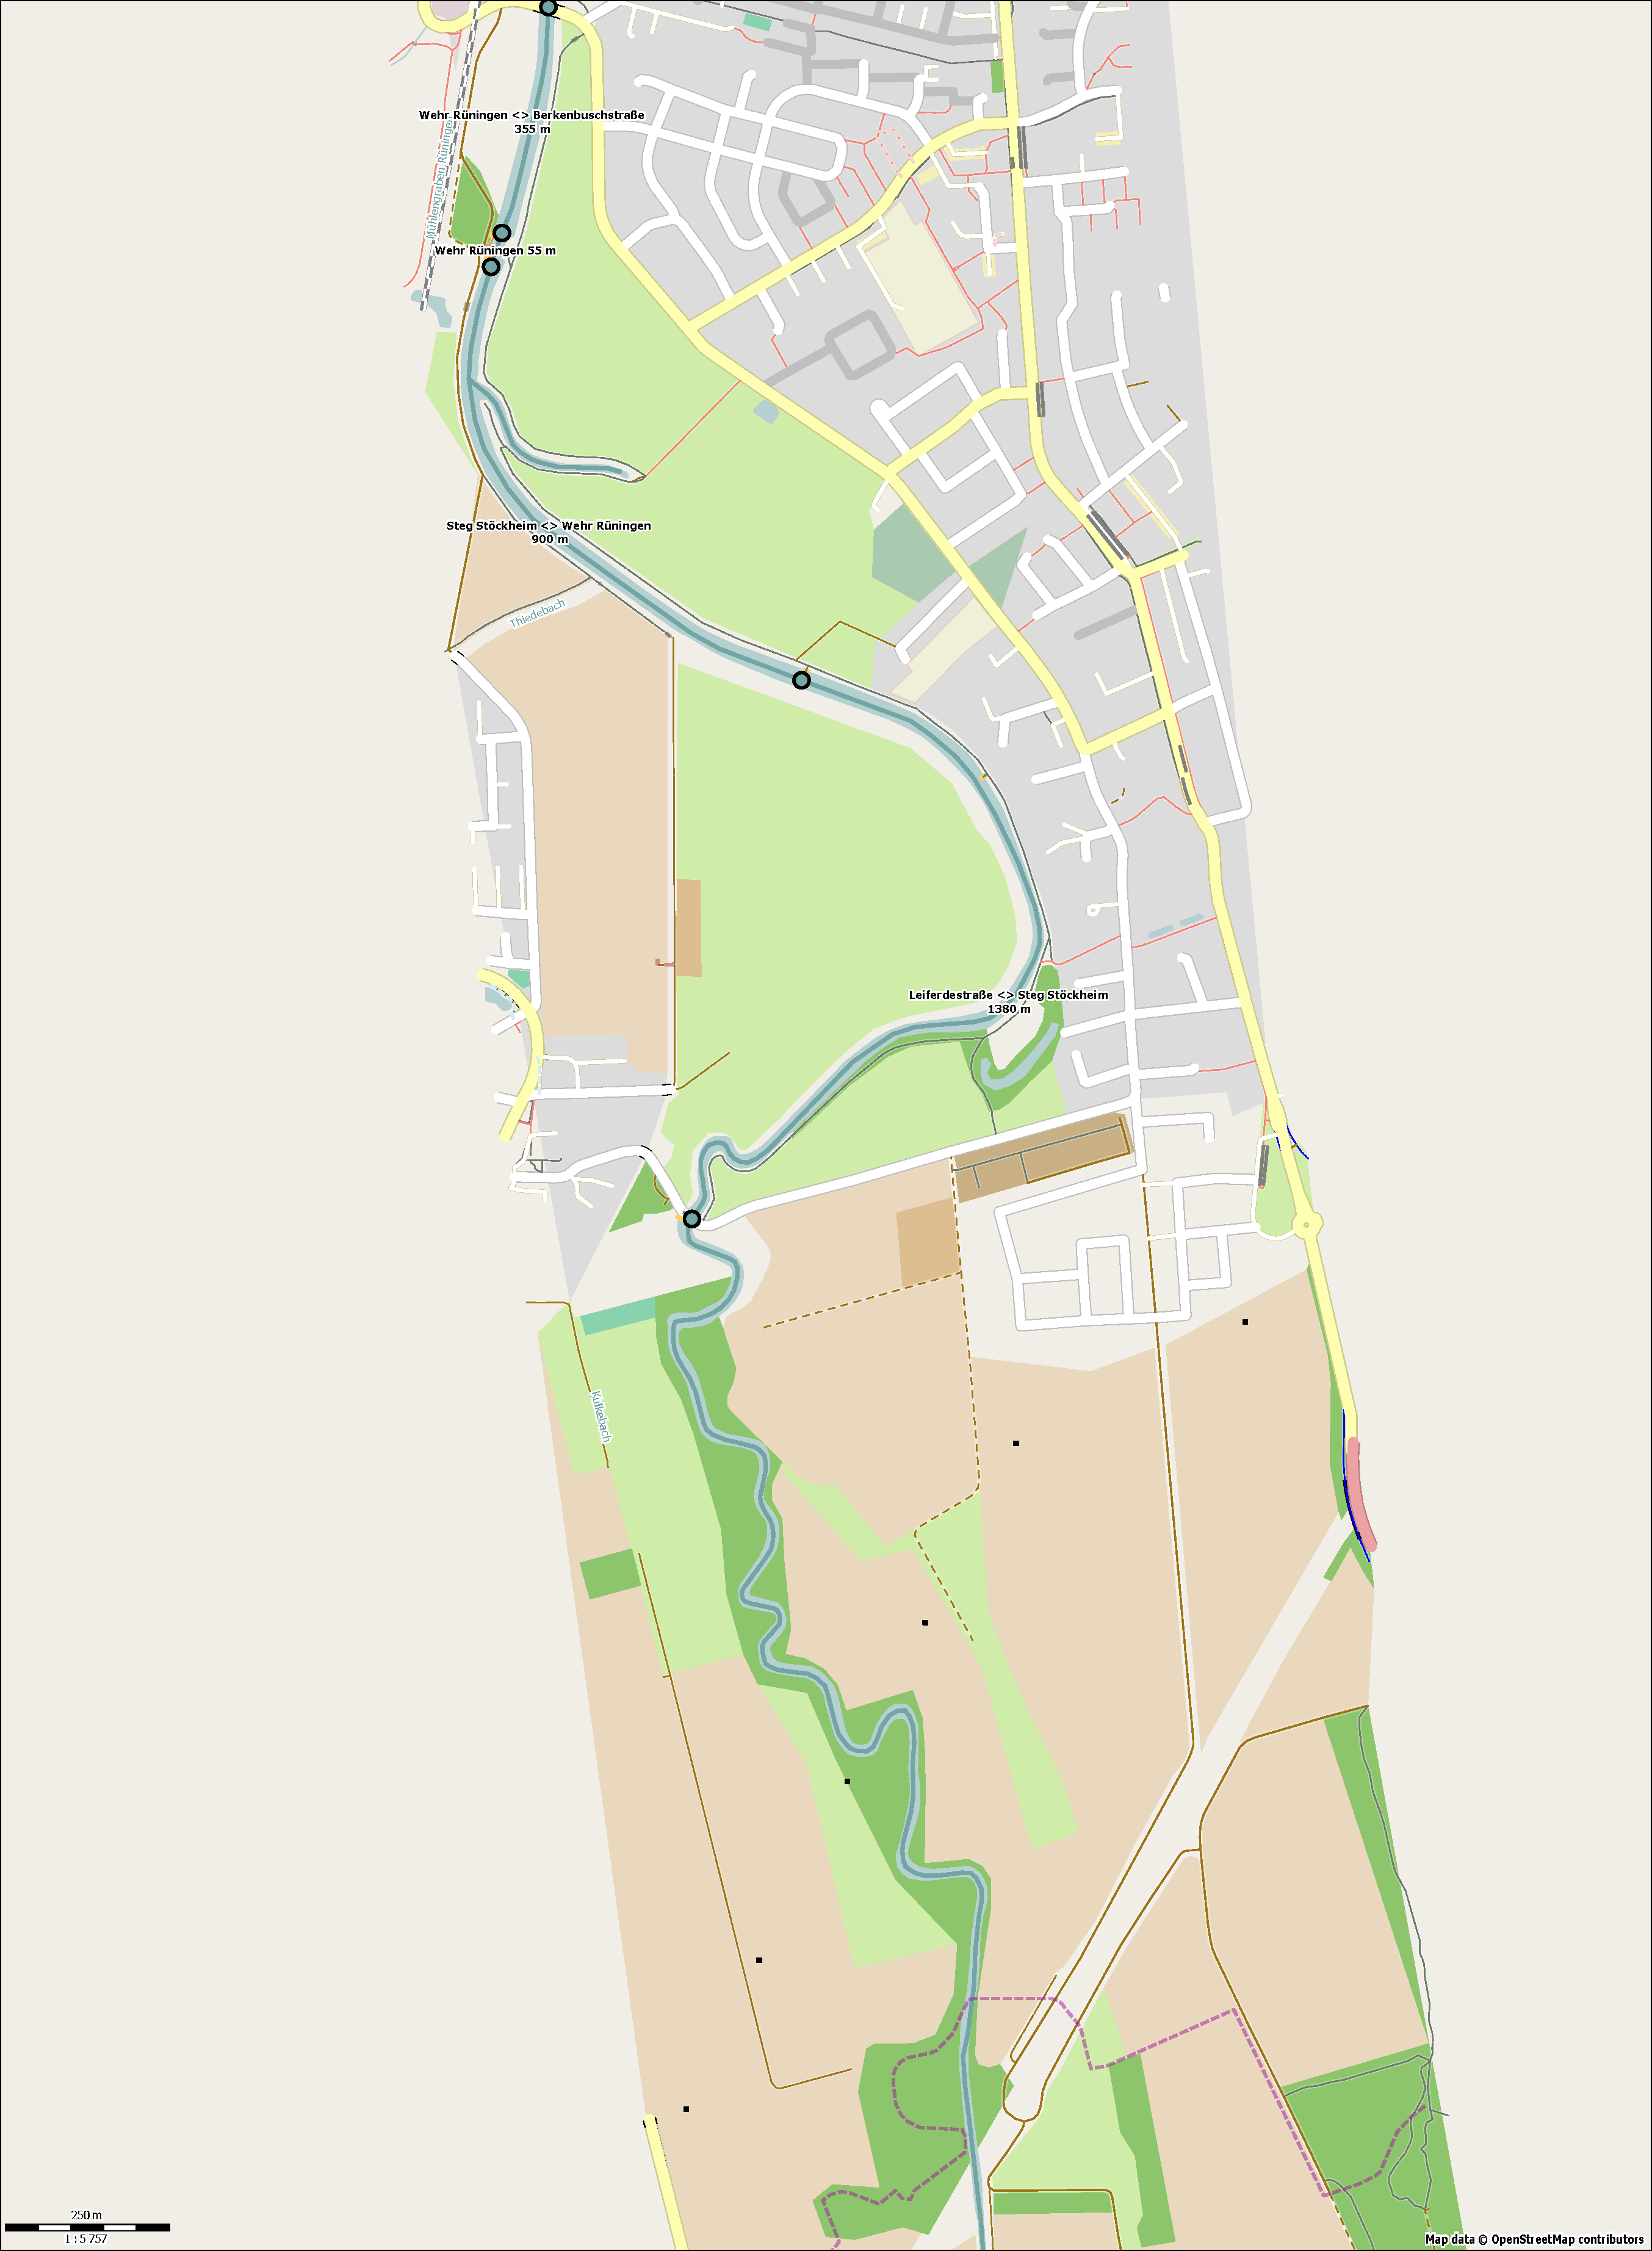
\includegraphics[max size={\textwidth}{\textheight}]{../Result/BS_Sued.pdf}
    \end{figure}
    \newpage
    
    \begin{figure}[!h]
        \centering
        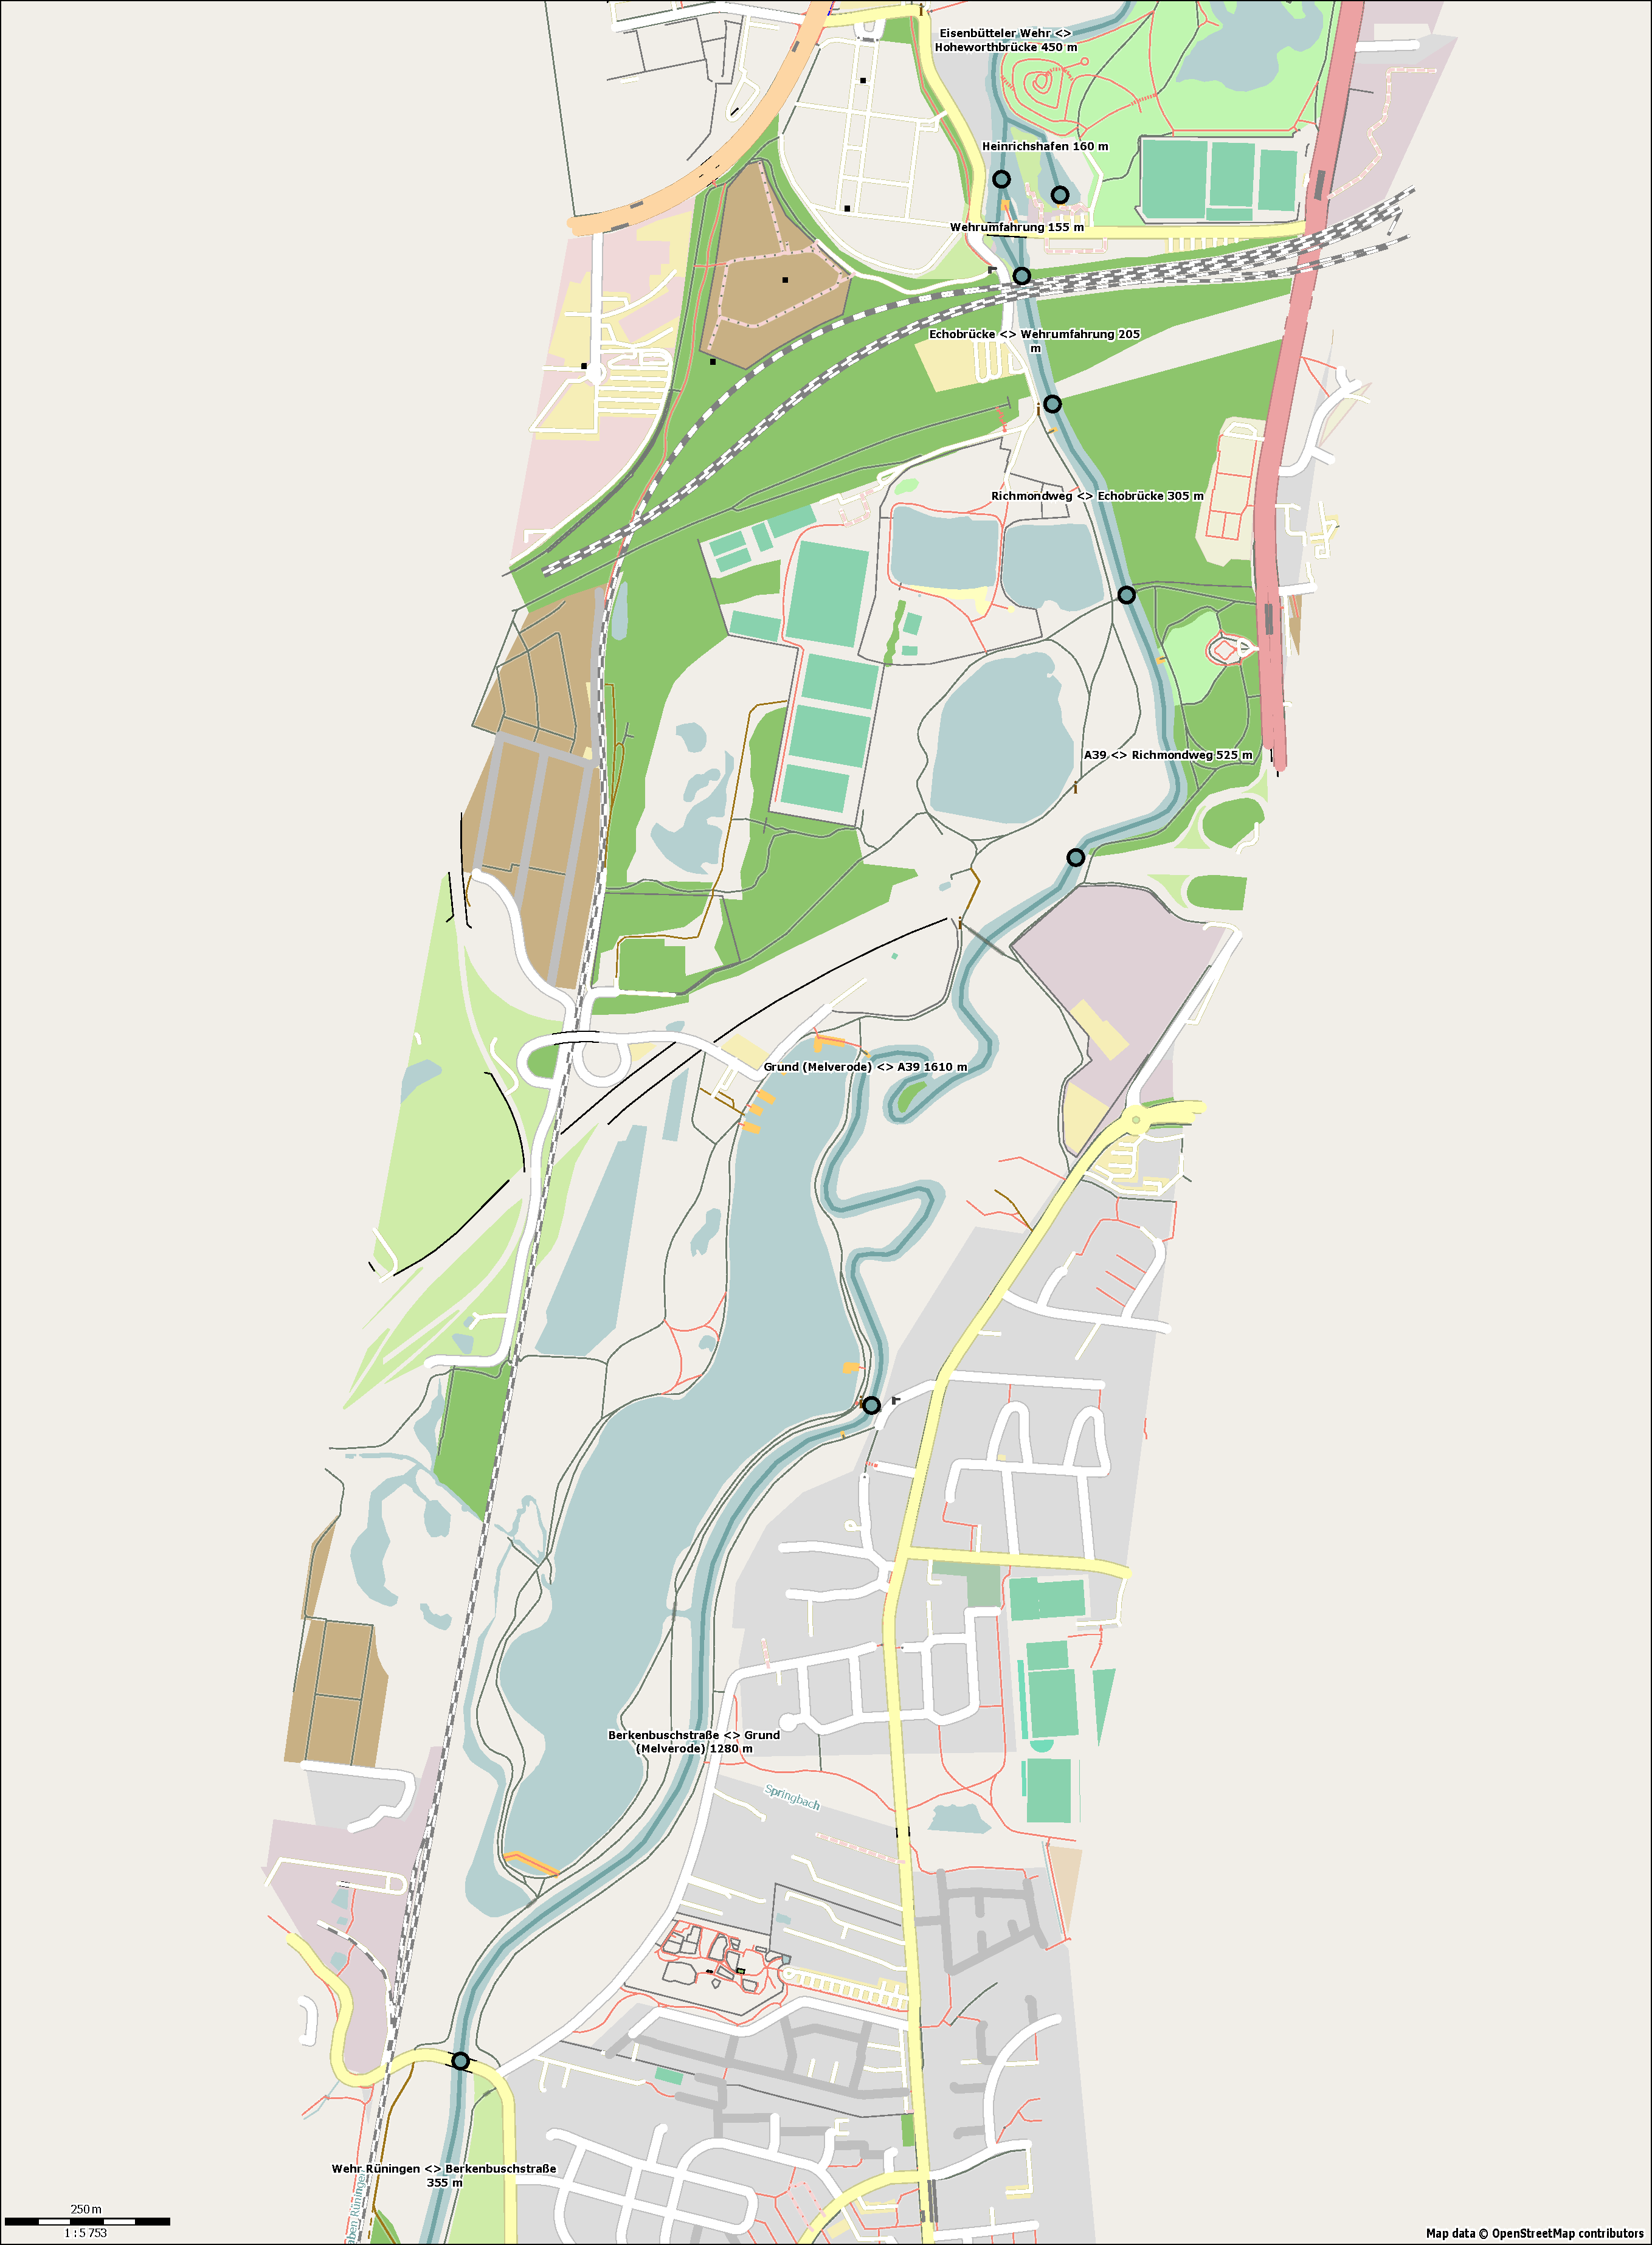
\includegraphics[max size={\textwidth}{\textheight}]{../Result/BS_Sued2.pdf}
    \end{figure}
    \newpage
    
    \begin{figure}[!h]
        \centering
        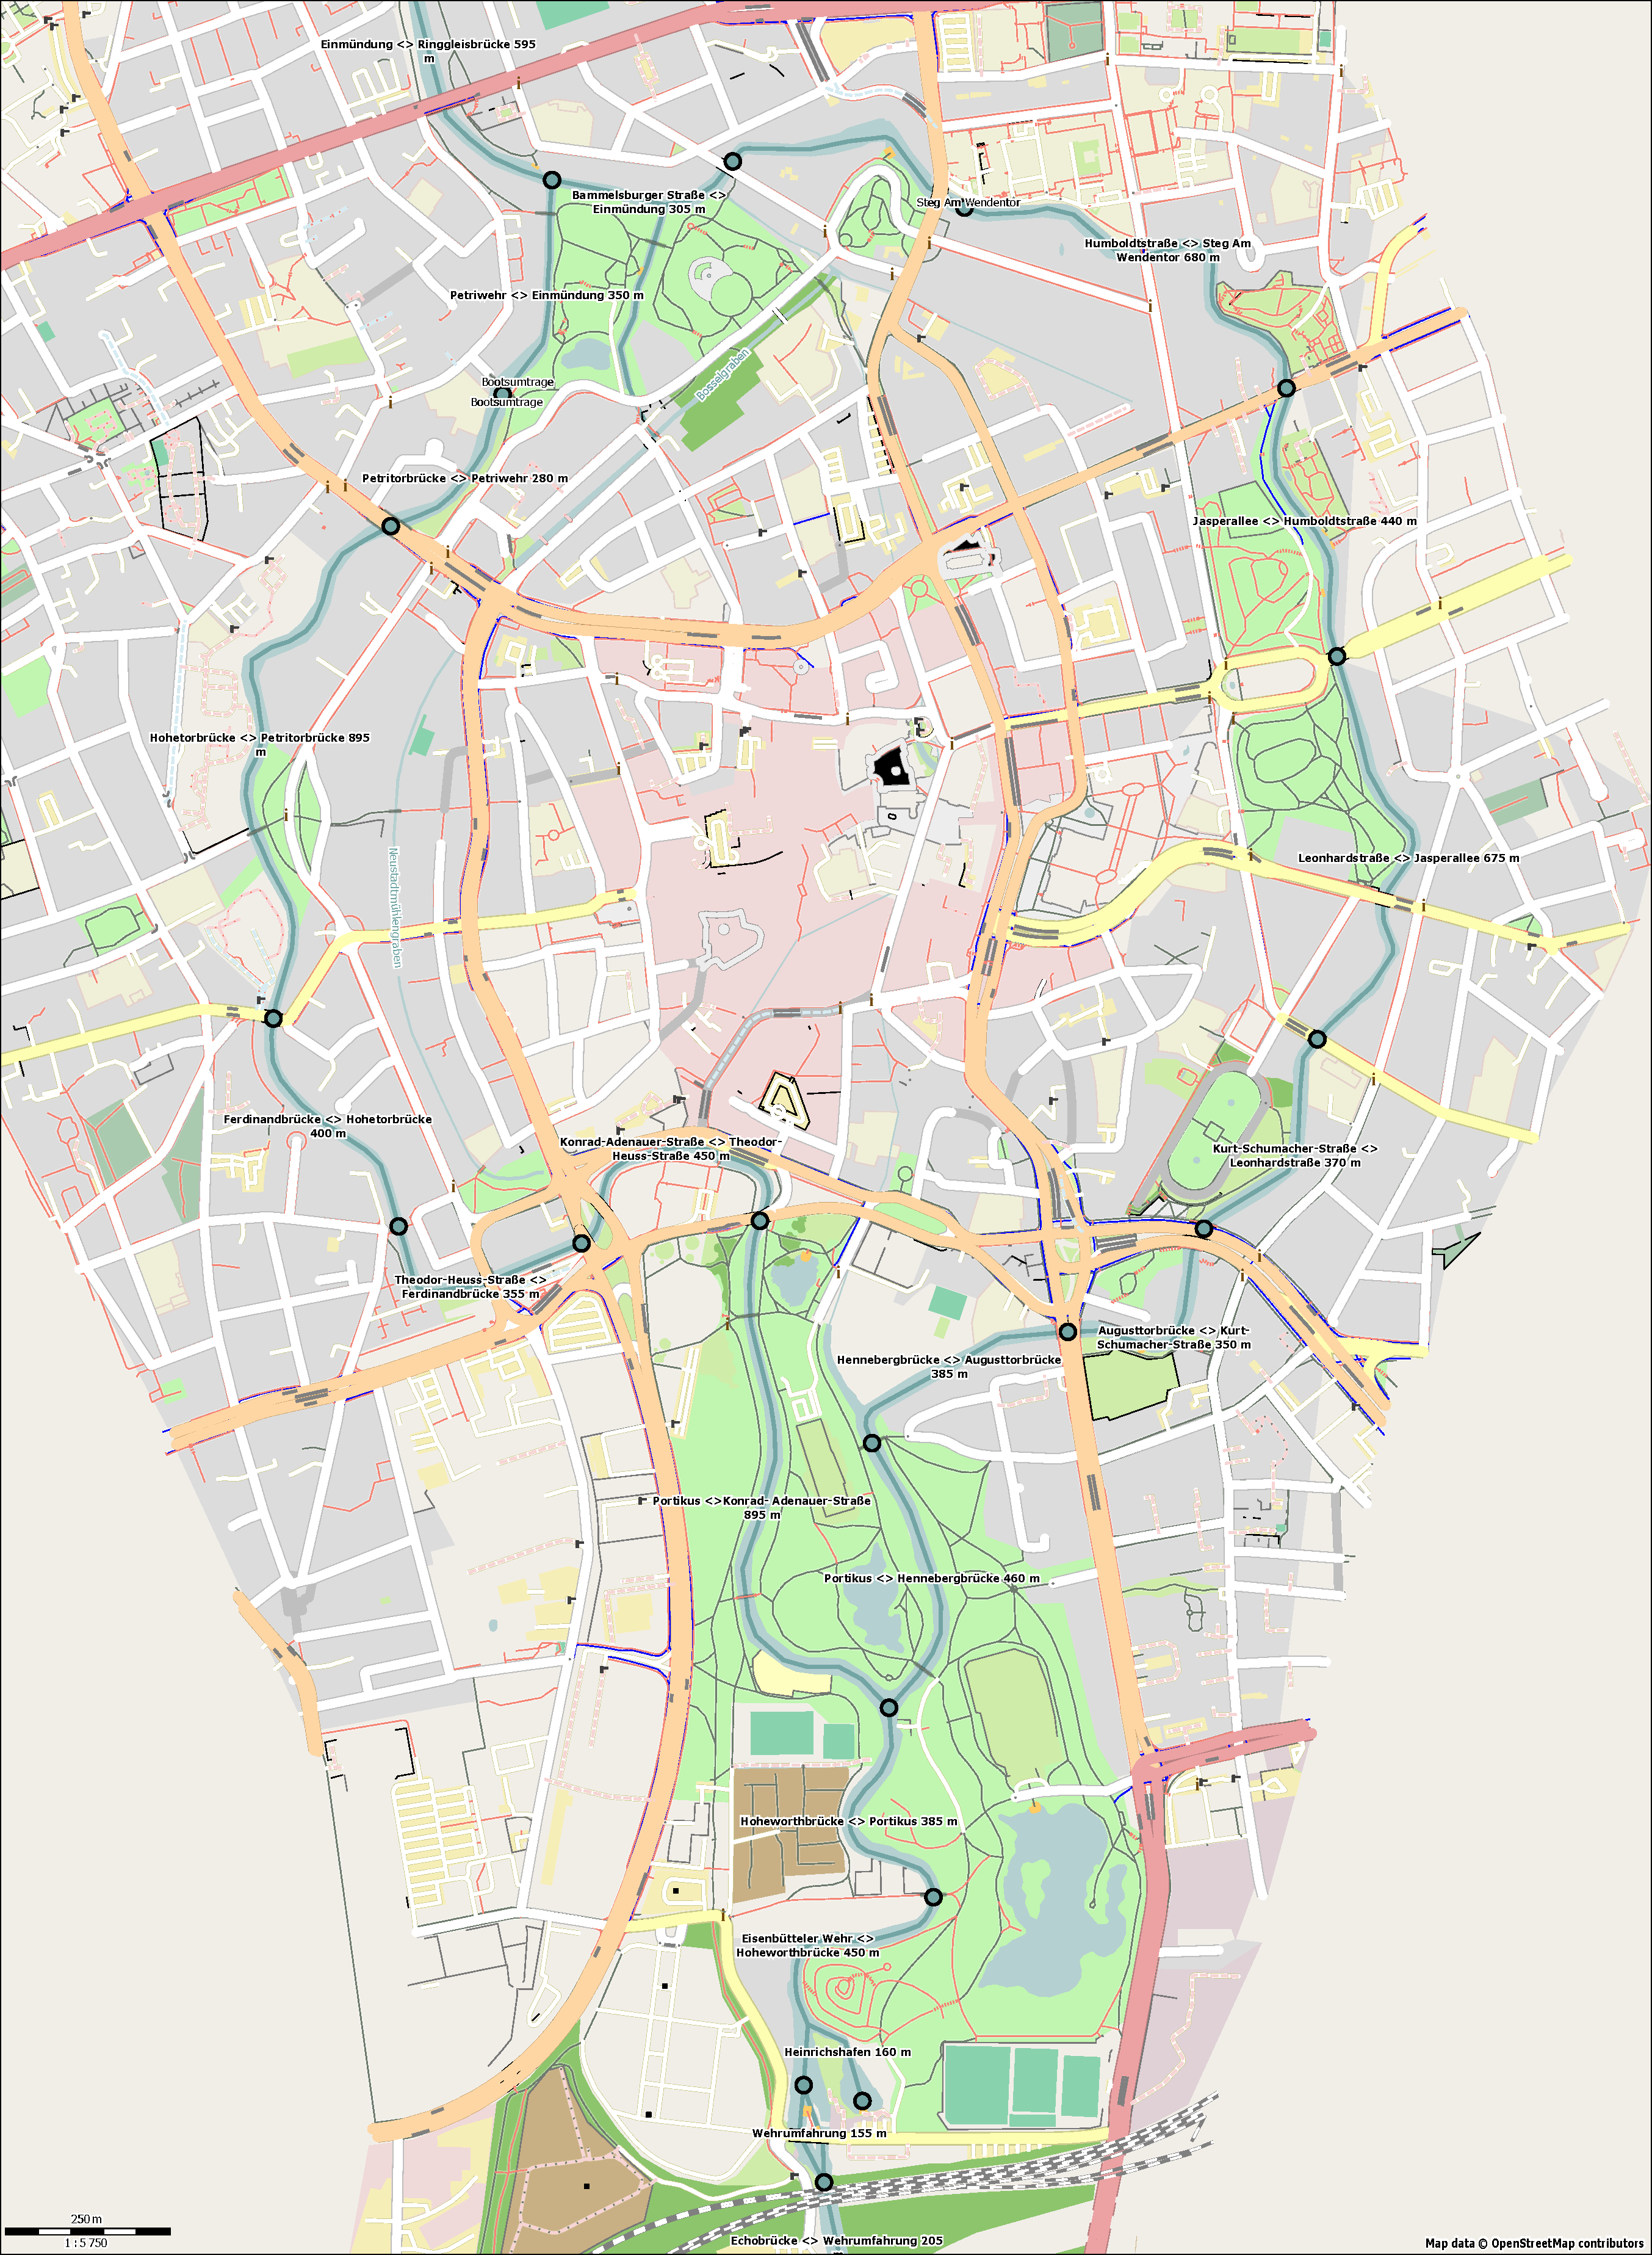
\includegraphics[max size={\textwidth}{\textheight}]{../Result/BS_Okerumflut.pdf}
    \end{figure}
    \newpage
    
    \begin{figure}[!h]
        \centering
        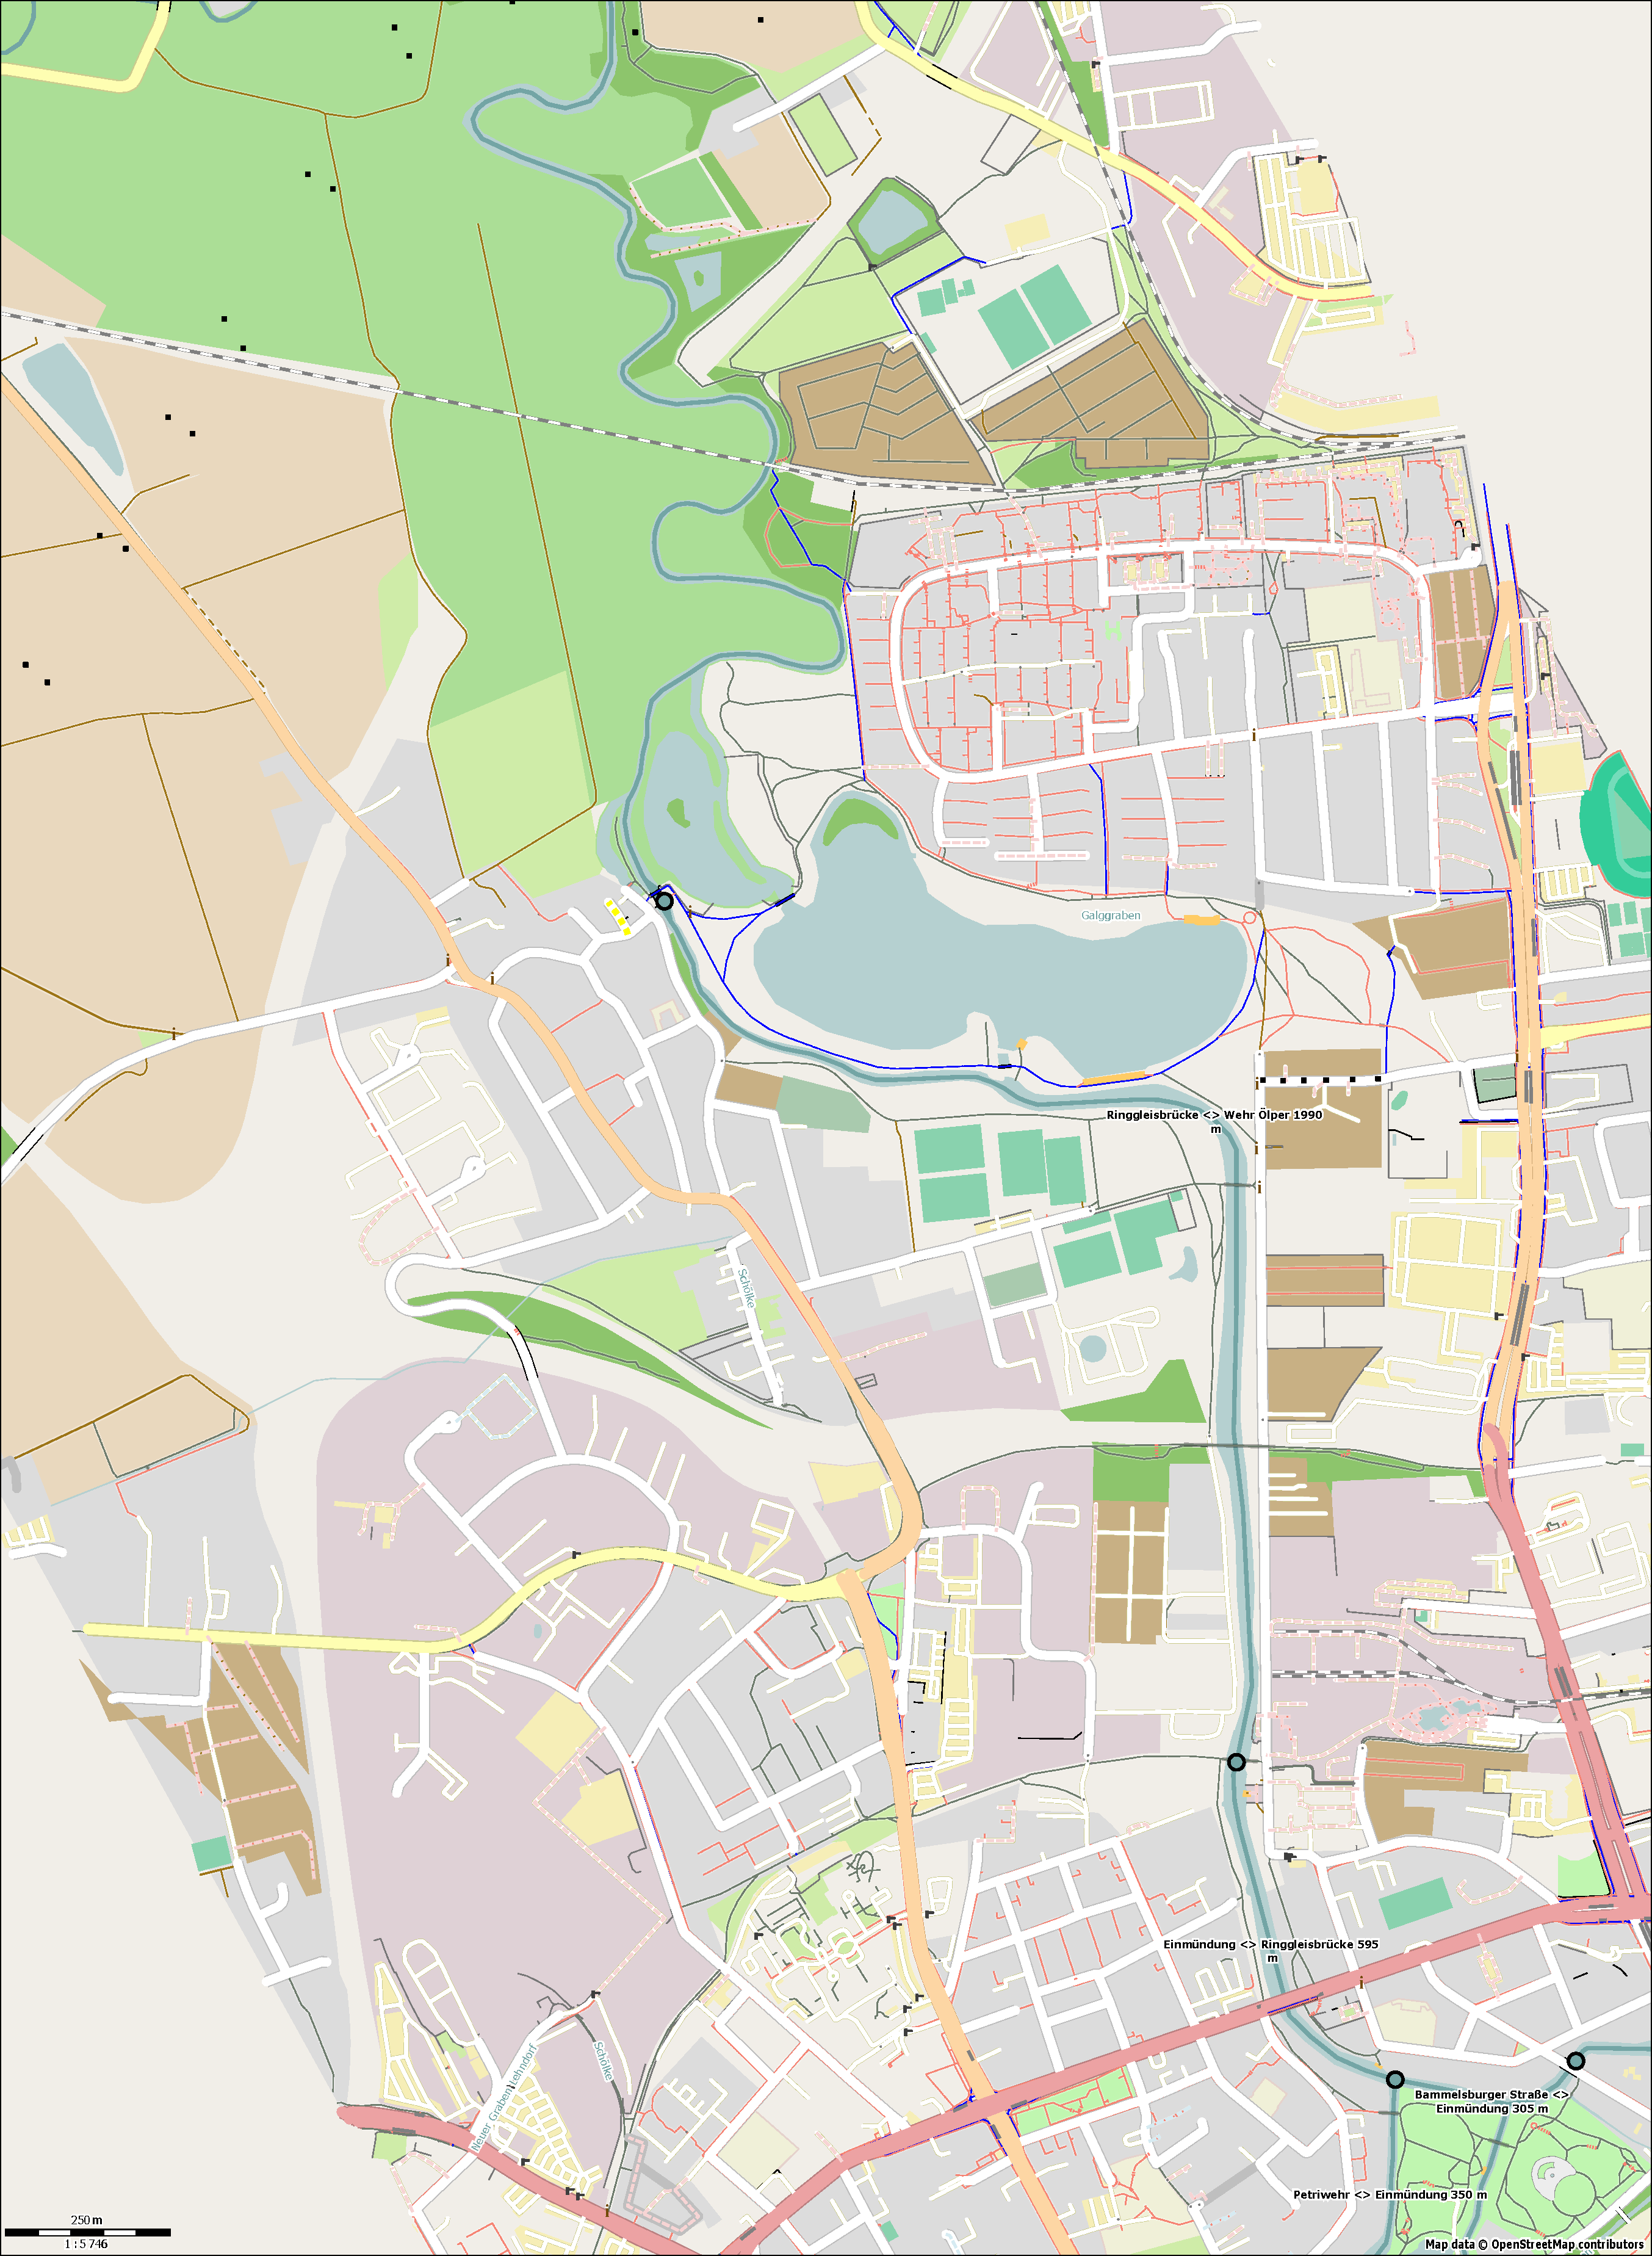
\includegraphics[max size={\textwidth}{\textheight}]{../Result/BS_Nord.pdf}
    \end{figure}
    \newpage
    
    \begin{figure}[!h]
        \centering
        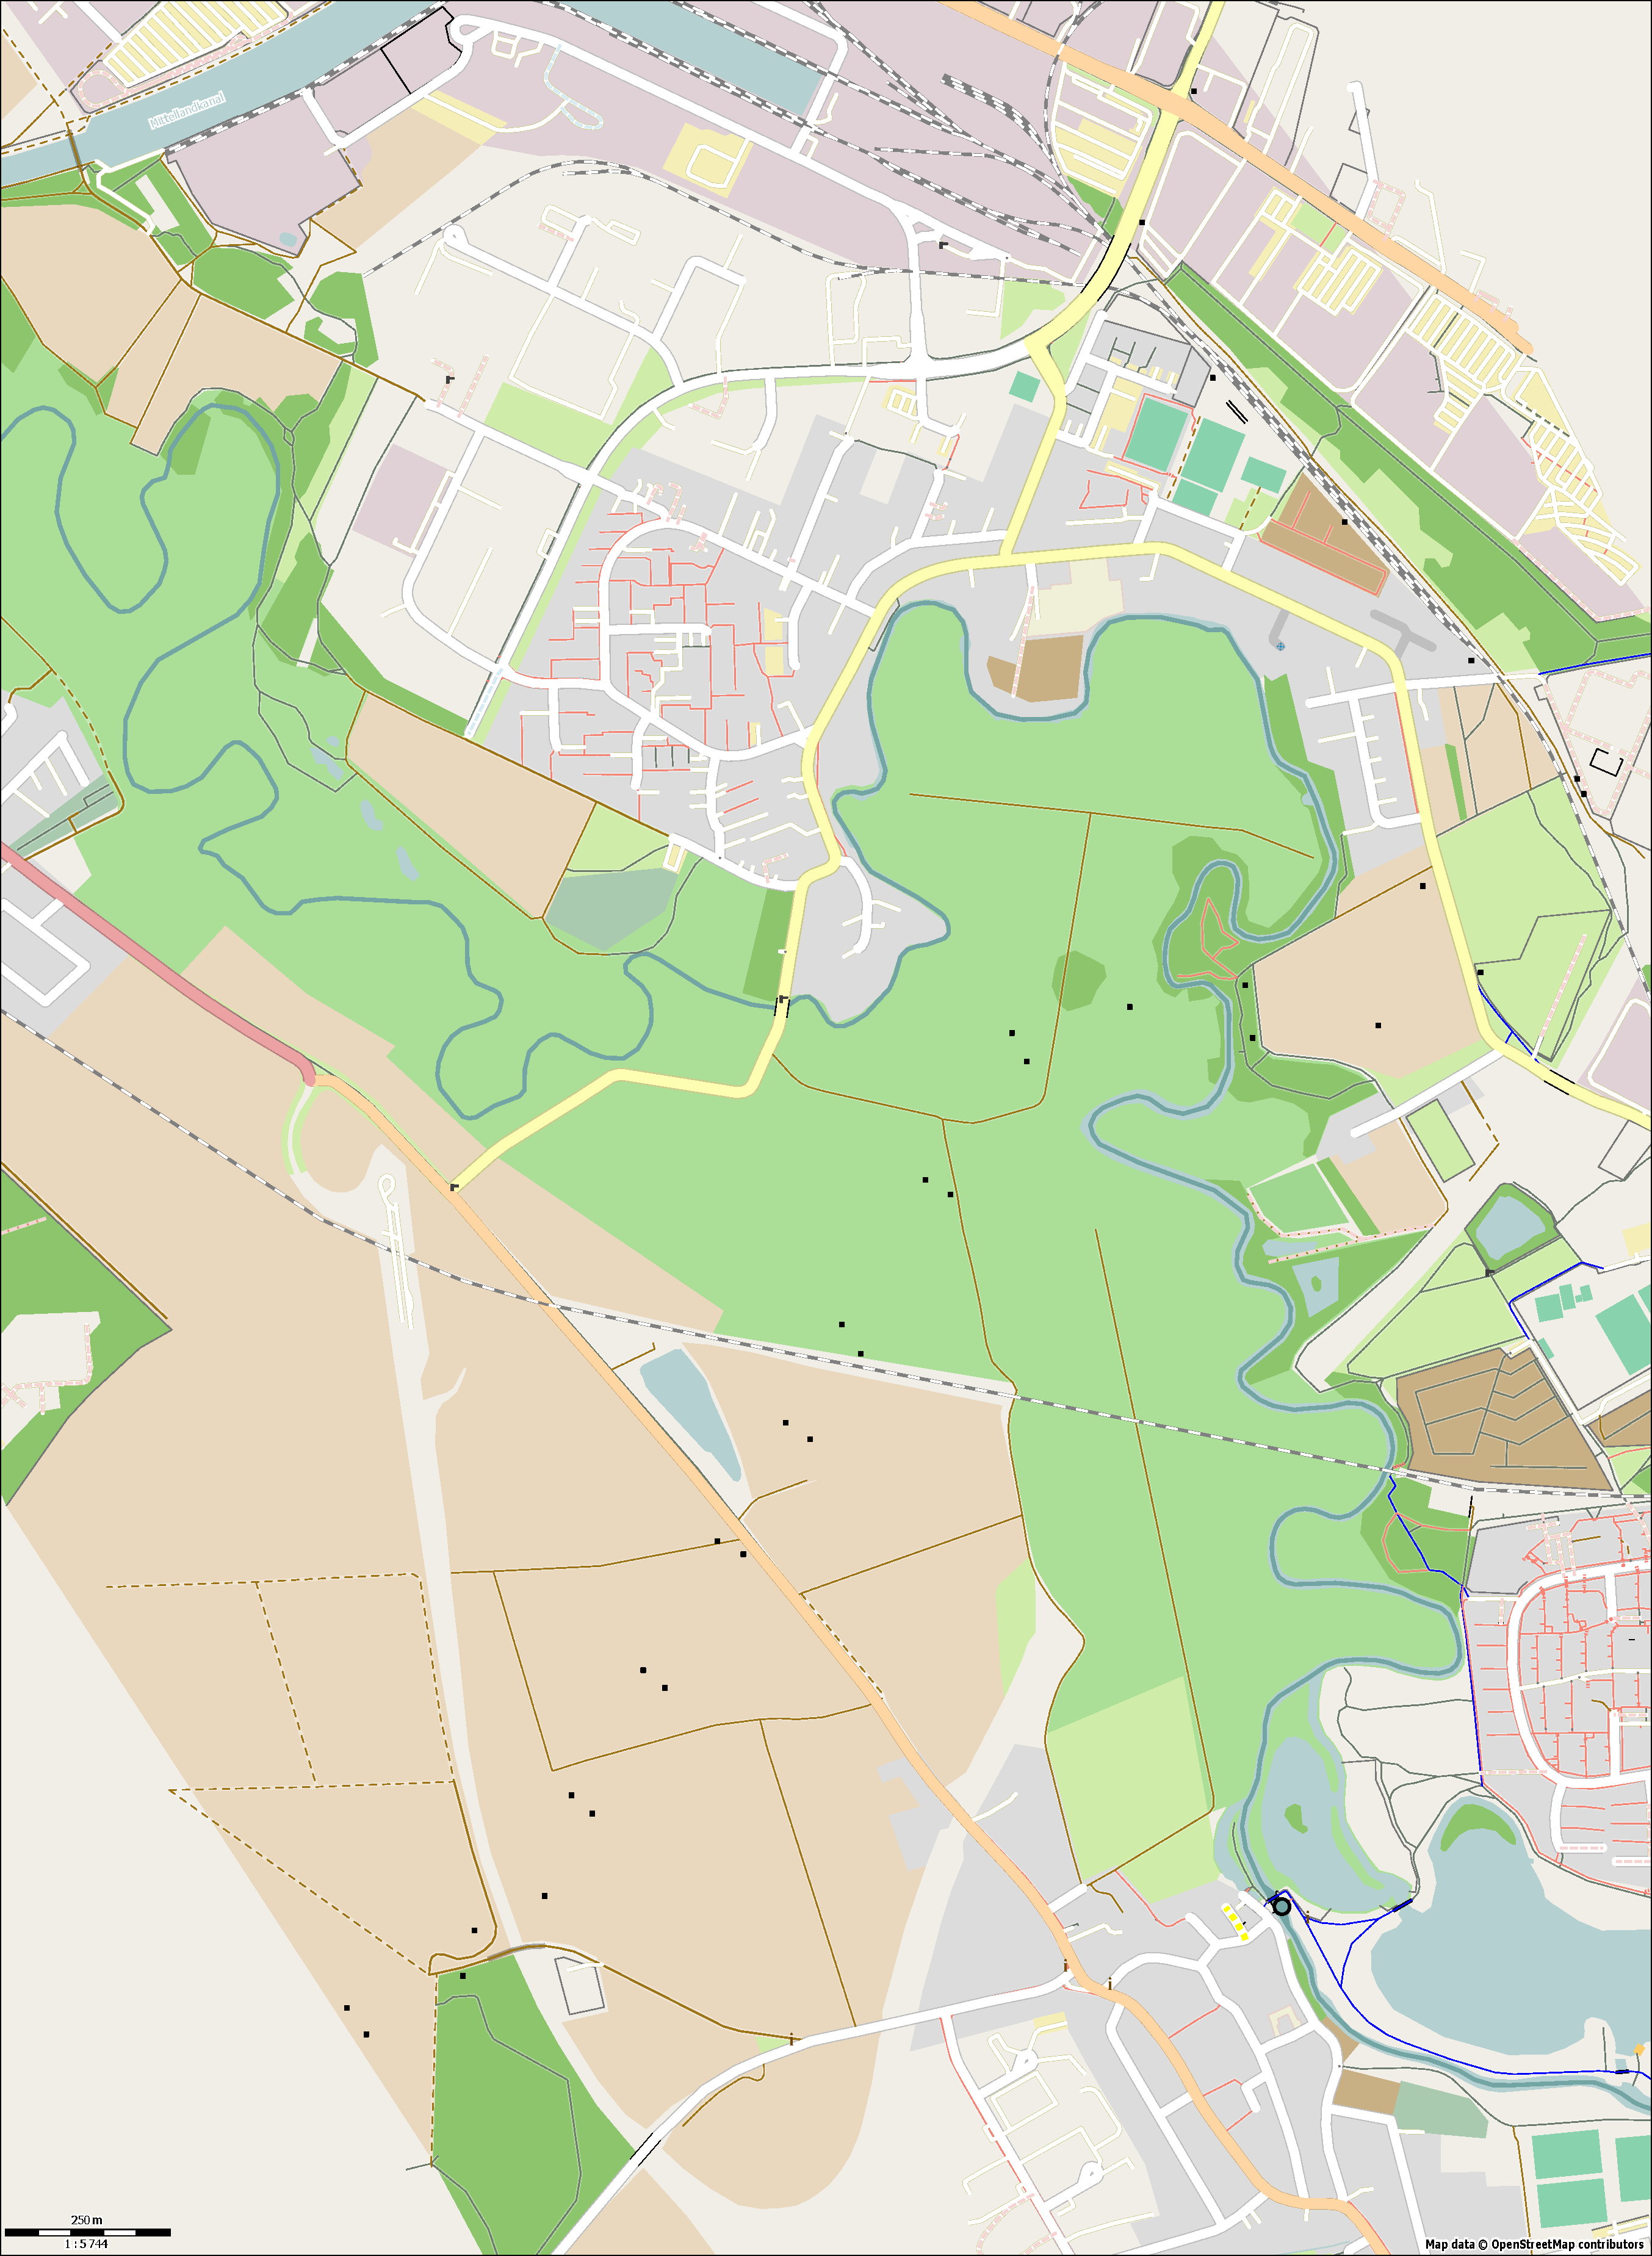
\includegraphics[max size={\textwidth}{\textheight}]{../Result/BS_Nord2.pdf}
    \end{figure}
    \newpage
    
    \begin{figure}[!h]
        \centering
        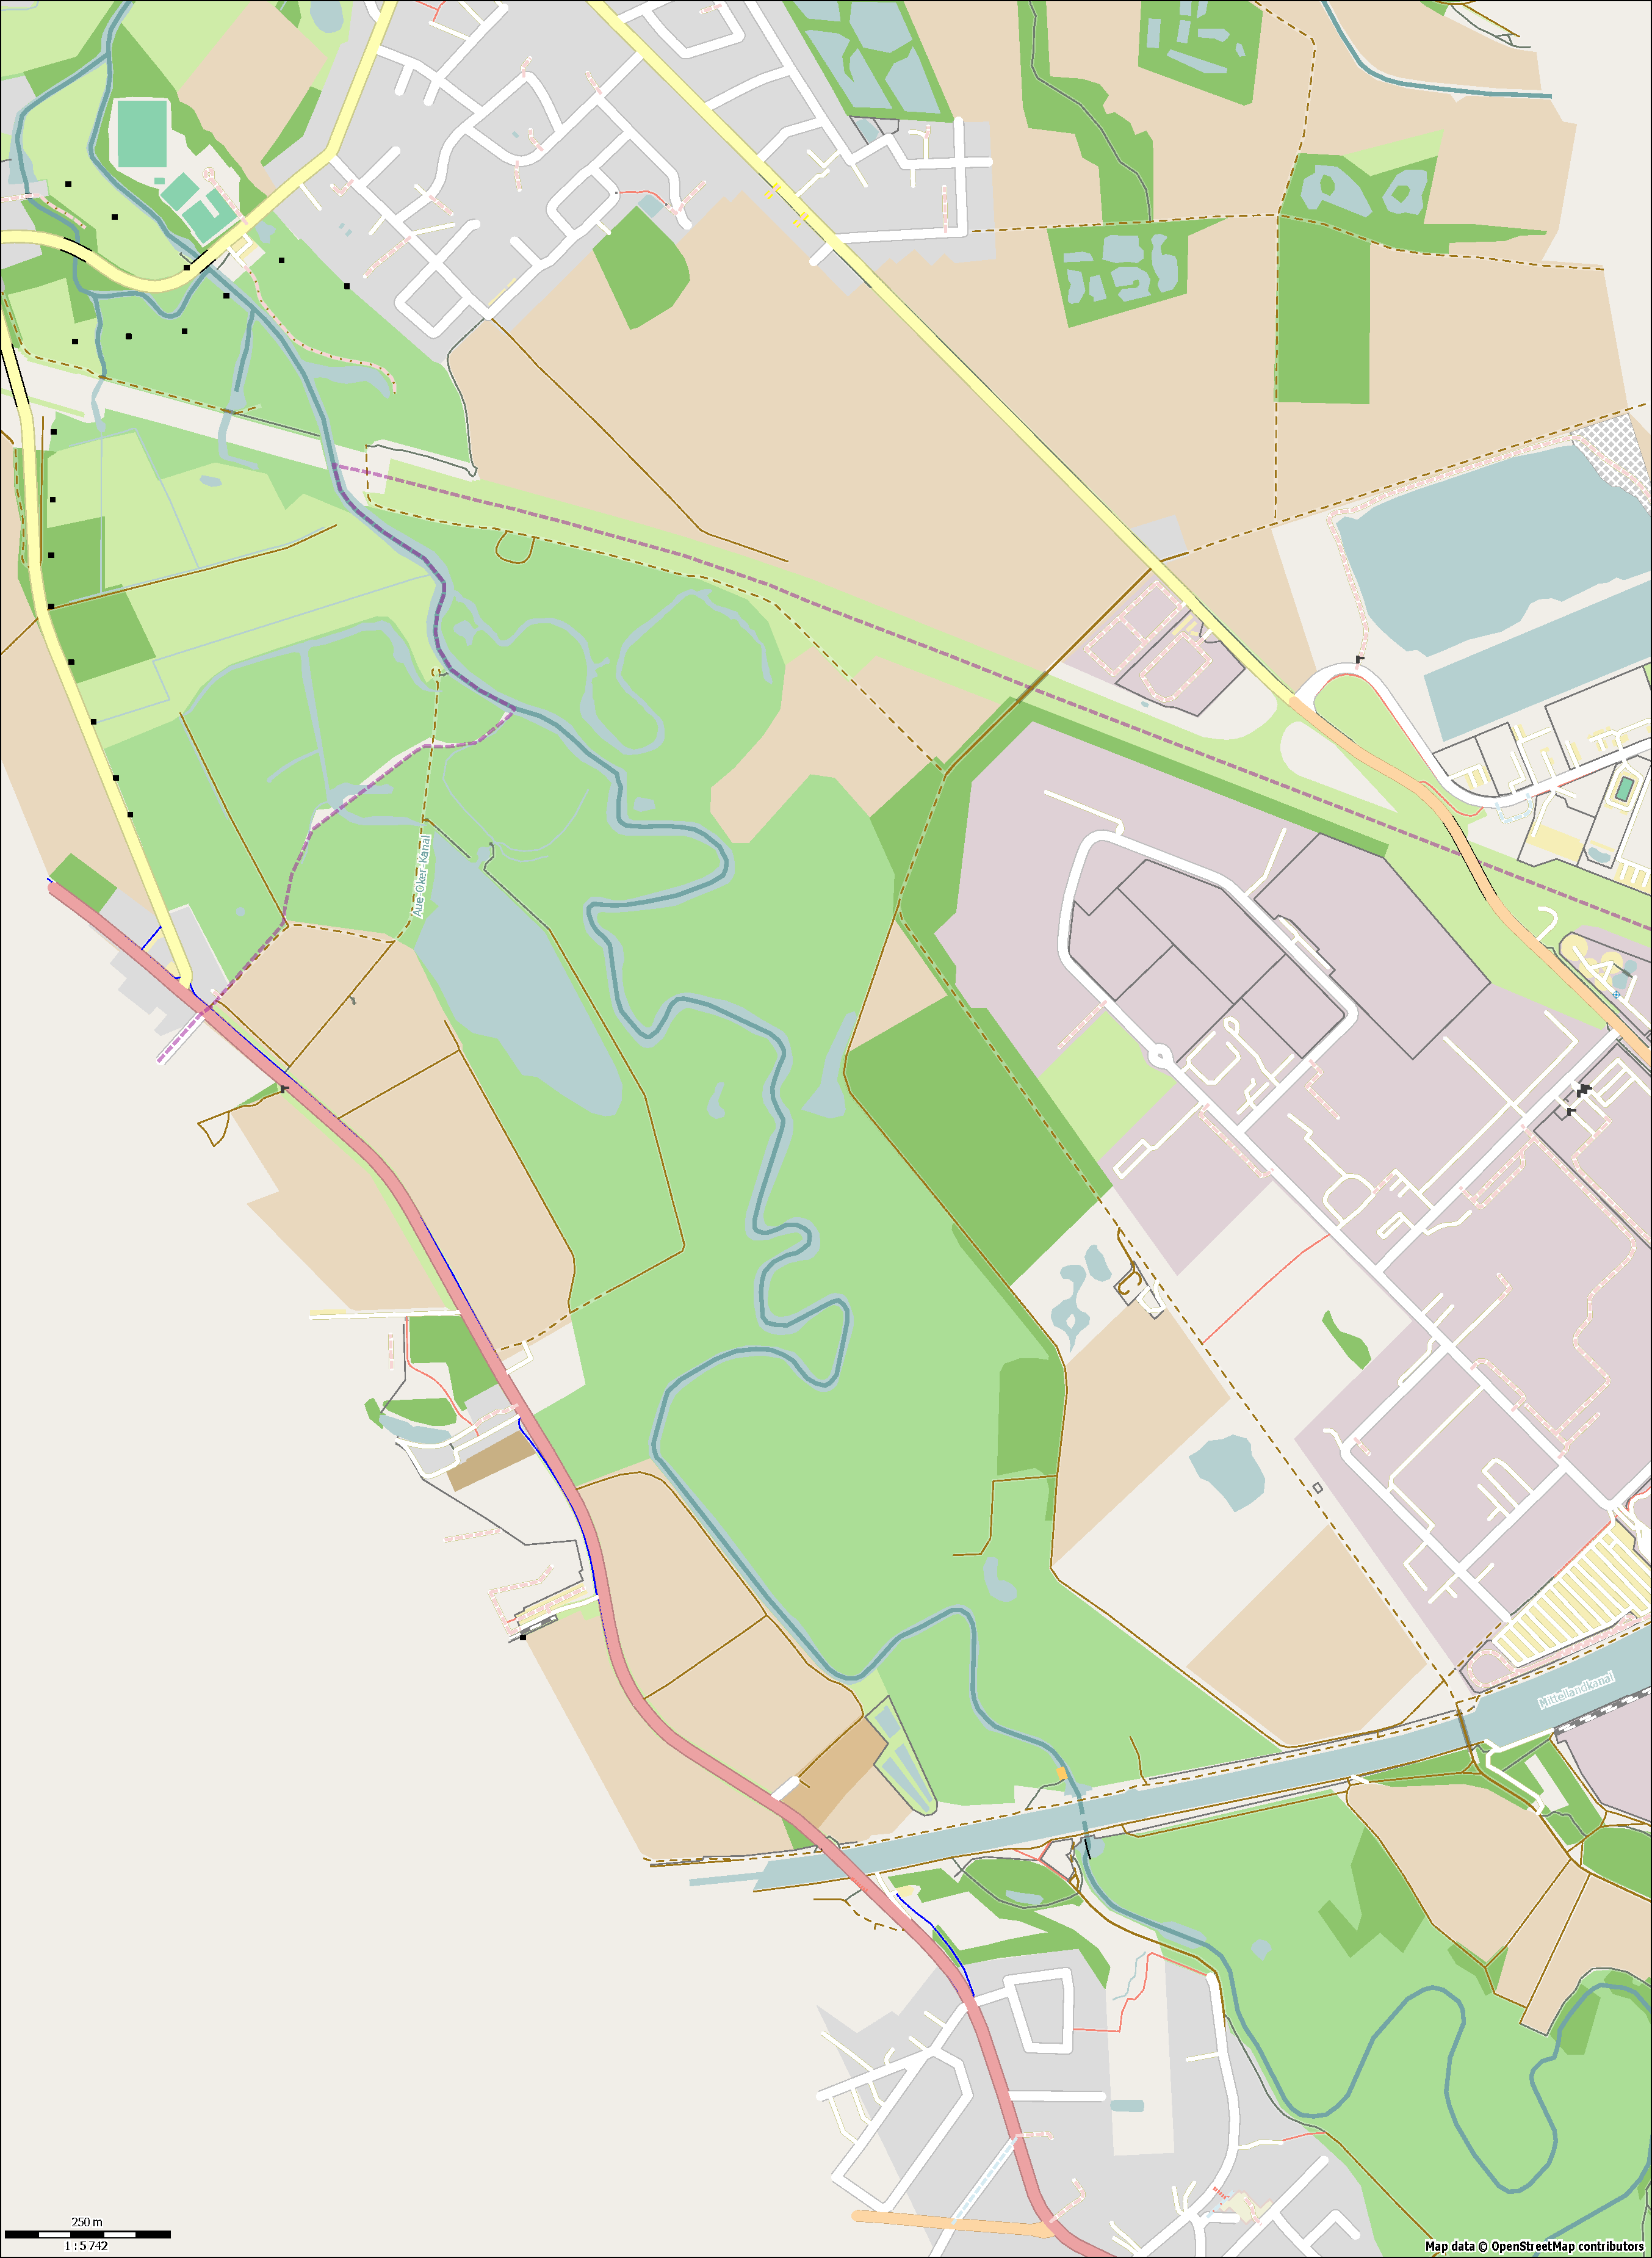
\includegraphics[max size={\textwidth}{\textheight}]{../Result/GF.pdf}
    \end{figure}
\end{document}